\section{Method} \label{sec:method} Prior work on anonymous \ac{dns} queries
has primarily focused on query latency when comparing against Tor-based
approaches~\cite{RFC9230,kurihara2023muodns,ODNS,xiao2025}. Such comparisons
typically assume the default Tor client configuration (e.g., in as in
DoHoT~\cite{DoHoT}), where circuits consists of three randomly selected relays
(see Section~\ref{sec:bg:tor}). The geographic placement of these relays can
heavily influence latency results. To provide a more complete picture, our
overarching evaluation considers additional dimensions such as the threat model
and deployability, in addition to exploring how we can reduce latency in
Tor-based solutions.

This study is focusing on two approaches for reducing latency in Tor circuits:
controlling the \emph{number} of relays and the \emph{location} of relays. The
default Tor configuration method (\texttt{torrc}) allows users to constrain the
geographic location of entry and exit relays via country codes, but offers no
control over the middle relay. It also does not support building circuits with
fewer than three relays. To overcome these limitations, the Python libraries
\texttt{carml}~\cite{carml} and \texttt{stem}~\cite{stem} are used, which
expose fine-grained control over circuit construction. With these tools, it is
possible specify country codes for the middle relay or omit it entirely (see
Figure~\ref{fig:carml-tor}), enabling the exploration of circuit configurations
that balance latency and anonymity systematically. 

\begin{figure}[h]
    \centering
    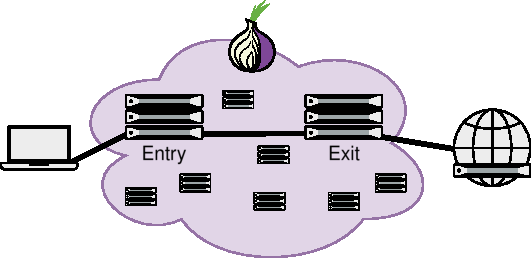
\includegraphics[width=\columnwidth]{img/dns-tor-carml.drawio.pdf}
    \caption{A Tor circuit created with carml and stem, using only an entry
    guard and an exit relay.}
    \label{fig:carml-tor}
\end{figure}

Since the client for the measurements is located in Sweden (country-code:
\texttt{se}), it is estimated that under normal routing conditions the Tor
relays in Sweden places them in close proximity to the client. In
Section~\ref{sec:limit} we address the limitations of Tor relay availability
around the world.

To eliminate the effects of caching and to maintain consistency across tests,
the measurements issue queries for uniquely generated \acp{sld} under a valid
\ac{tld}, which are expected to return an non-existing-domain return code
(NXDOMAIN). The query name consists of
\texttt{prot-method-circuit-i-XXXXXXXX.net}. The first part is the protocol in
use (i.e, dohot, dotor, odoh). The second part is the method for building
circuits (i.e., torrc or carml). The third part represents the built circuit
using the country codes for each relay. A circuit consisting of three
unspecified relays is represented as: \texttt{any2any2any}, while a two relay
circuit contstrained to Sweden is represented as: \texttt{se2se}. In addition
to these parameters an increasing number representing the measurement index
(0-999) as well as a random alphanumeric string are included to ensure that the
query is unique to avoid influence of cache hits. This approach with unique
NXDOMAIN queries ensures that the observed latency mainly reflects the path
between the client and the resolver.

Each configuration is measured 1,000 times with unqiue queries. In each
iteration, we start our measurement container with the specified configuration
and wait until a circuit is established and an arbitrary query receives a
successful response. This prelude ensures that the Tor circuit is fully
established and that we have a functional \ac{dns} resolution over Tor. A query
is then issued for an A record using a unique non-existent domain described
earlier, and the time for the reply to return is measured in milliseconds.
Finally, the container is stopped before the next iteration begins to ensure a
new circuit. The code for the containers and measurement script can be found on
GitHub\footnote{Anonymized for submission}.

For comparison we set up docker containers running \ac{dohot} and
\ac{odoh}. Both of these utilize DNSCrypt-proxy which is a flexible proxy for
\ac{dns} and supports many encryption protocols~\cite{dnscrypt-proxy}.
DNSCrypt-proxy is responsible for listening on a port for client queries and
sending them to the configured anonymization approach. For \ac{odoh} we choose
a proxy in Sweden to mimic the tuned circuit in \ac{dohot}. We decided to pick
a single \ac{doh} provider for our measurements to limit the number of
variables. Our choice of \ac{doh} resolver, Cloudflare's \texttt{1.1.1.1}, is
using anycast which means that the closest from the perspective of our exit or
proxy will be used\footnote{\url{https://developers.cloudflare.com/1.1.1.1/}}.

In addition we also implemented and measured the latency of \ac{dotor}. This is
similar to the Tor-based approach used for comparison with
\ac{odns}~\cite{ODNS} where \ac{doh} is not used. Instead the query is resolved
by the exit relay. Our \ac{dotor} approach relies on directly interfacing with
the Tor client using its extensions to the SOCKS5 protocol, specifically the
RESOLVE command value (0xF0)\cite{tor-socks5}. This allows for sending a domain
to be resolved instead of a destination for the exit relay to connect to. It
should be noted that this approach does not utilize full \ac{dns}-queries at
this level. To interface with the Tor client a python script is instead
utilized to receive and provide dig-compliant DNS queries and their answers.
While negligible in this context, it should be noted that some overhead is
incurred in the process.


